\documentclass[11pt]{article}

% Standard arXiv-compatible packages
\usepackage[utf8]{inputenc}
\usepackage[T1]{fontenc}
\usepackage{geometry}
\geometry{a4paper, margin=1in}
\usepackage{mathtools}  % Loads amsmath automatically
\usepackage{amssymb}
\usepackage{amsthm}
\usepackage{graphicx}
\usepackage{mathrsfs}
\usepackage{xcolor}
\usepackage{tikz}
\usetikzlibrary{arrows.meta, positioning, matrix, decorations.pathreplacing}
\usepackage{booktabs}
\usepackage{caption}
\usepackage{enumitem}
\usepackage{braket}
\usepackage{comment}
\usepackage[hidelinks]{hyperref}
\usepackage{microtype}
\usepackage{cleveref}
\usepackage{algorithm}
\usepackage{algpseudocode}

% Custom commands
\newcommand{\tr}{\operatorname{tr}}
\newcommand{\expm}{\operatorname{expm}}
\newcommand{\diag}{\operatorname{diag}}
\newcommand{\R}{\mathbb{R}}
\newcommand{\C}{\mathbb{C}}
\newcommand{\N}{\mathbb{N}}
\newcommand{\order}[1]{\mathcal{O}(#1)}

% Theorem environments
\newtheorem{theorem}{Theorem}
\newtheorem{proposition}[theorem]{Proposition}
\newtheorem{lemma}[theorem]{Lemma}
\newtheorem{corollary}[theorem]{Corollary}
\theoremstyle{definition}
\newtheorem{definition}[theorem]{Definition}
\newtheorem{example}[theorem]{Example}
\theoremstyle{remark}
\newtheorem{remark}[theorem]{Remark}

% Number theorems by section
\numberwithin{theorem}{section}
\numberwithin{equation}{section}

% Bibliography setup
\usepackage[backend=biber,style=alphabetic,natbib=true]{biblatex}
\addbibresource{block-matrix-exponentials.bib}

\captionsetup{font=small}

\begin{document}

\title{Block Matrix Exponentials as Generating Functions\\for Time-Ordered Perturbations}

\author{Neil D. Lawrence\\
University of Cambridge\\
\texttt{neil@someaddress.ac.uk}}

\date{\today}

\maketitle

\begin{abstract}
We explore the connection between structured block matrix exponentials and time-ordered integral operators arising in quantum perturbation theory, path integrals, and information geometry. We observe that off-diagonal blocks of $\exp(M)$ for block upper-triangular matrices $M$ compute sums over time-ordered insertions of perturbations, with different block topologies yielding different orderings. We explicitly interpret Higham's $4n \times 4n$ construction as computing symmetric second Fr\'echet derivatives (summing over both time orderings), while the Najfeld--Havel $3n \times 3n$ construction captures single-ordered products corresponding to causal propagation. This perspective provides: (1) an algebraic interpretation of time ordering as an emergent property of matrix block structure; (2) a systematic approach to computing Fr\'echet derivatives, Fisher information in quantum exponential families, and Dyson series terms using existing matrix exponential algorithms; and (3) a unifying framework connecting numerical linear algebra, quantum field theory, and statistical geometry. We demonstrate computational advantages over nested quadrature with numerical benchmarks on quantum spin systems, showing 10--100$\times$ speedups while maintaining stability and accuracy.
\end{abstract}

\tableofcontents

\section{Introduction}
\label{sec:introduction}

\subsection{Motivation}
\label{subsec:motivation}

Time-ordered integrals appear ubiquitously across mathematics and physics:
\begin{itemize}[leftmargin=*]
\item In quantum mechanics, the Dyson series represents time evolution under a time-dependent perturbation as a sum of time-ordered integrals~\cite{Dyson-radiation49}.
\item In quantum field theory, propagators and correlation functions require time-ordering operators to ensure causality~\cite{peskin1995introduction}.
\item In statistical physics, linear response theory and Kubo formulas express susceptibilities as time-ordered correlators~\cite{kubo1957statistical}.
\item In information geometry, the Fisher metric for exponential families involves second derivatives of the log-partition function, which correspond to symmetric time-ordered integrals~\cite{amari2016information}.
\item In numerical analysis, Fr\'echet derivatives of matrix functions require nested integrals that respect ordering~\cite{higham2008functions}.
\end{itemize}

Standard approaches to computing these integrals typically involve either:
\begin{enumerate}
\item \textbf{Explicit time-ordering operators} (in physics), which require careful bookkeeping of operator orderings and lead to combinatorially complex expressions at higher orders, or
\item \textbf{Nested numerical quadrature} (in numerical analysis), which scales poorly with the number of insertions and can suffer from stability issues.
\end{enumerate}

This paper makes explicit a connection implicit in existing work: \emph{block matrix exponentials serve as generating functions for time-ordered perturbations}. Off-diagonal blocks of $\exp(M)$ for structured block matrices $M$ automatically encode sums over insertion times, with the block topology determining which time orderings contribute. This observation provides both a conceptual unification---time ordering emerges from algebraic structure---and a systematic computational approach that leverages highly optimized matrix exponential routines.

\subsection{Main Results}
\label{subsec:main_results}

Our key insight is summarized in the following informal statement:

\begin{quote}
\emph{The off-diagonal blocks of $\exp(M)$ for block upper-triangular $M$ encode sums over all paths through the block structure. Each path corresponds to a specific time ordering of marked perturbations. Different block topologies select different subsets of orderings.}
\end{quote}

We present three key formulas (drawn from Higham and Najfeld--Havel) with their time-ordering interpretation:

\begin{enumerate}[leftmargin=*]
\item \textbf{First-order formula} (\Cref{thm:first_order}): For a $2n \times 2n$ block matrix
\[
M = \begin{bmatrix} H & V \\ 0 & H \end{bmatrix},
\]
the $(1,2)$ block of $\exp(M)$ equals the integral
\[
L(H,V) = \int_0^1 e^{(1-s)H} V e^{sH} \, ds,
\]
which is the first-order term in the Dyson series.

\item \textbf{Symmetric second-order formula} (\Cref{thm:higham_symmetric}): Using Higham's $4n \times 4n$ construction
\[
M = \begin{bmatrix} H & E_1 & E_2 & 0 \\ 0 & H & 0 & E_2 \\ 0 & 0 & H & E_1 \\ 0 & 0 & 0 & H \end{bmatrix},
\]
the $(1,4)$ block equals
\[
L^{(2)}(H; E_1, E_2) = \int_0^1 \int_0^{s_2} e^{(1-s_2)H} E_2 e^{(s_2-s_1)H} E_1 e^{s_1 H} \, ds_1 \, ds_2 + (E_1 \leftrightarrow E_2),
\]
the symmetric second Fr\'echet derivative of $\exp(H)$.

\item \textbf{Causal second-order formula} (\Cref{thm:najfeld_havel_causal}): Using the Najfeld--Havel $3n \times 3n$ construction
\[
M = \begin{bmatrix} H & E_1 & 0 \\ 0 & H & E_2 \\ 0 & 0 & H \end{bmatrix},
\]
the $(1,3)$ block captures only the ordering $s_1 < s_2$, corresponding to a time-ordered (causal) product.
\end{enumerate}

\Cref{tab:block_comparison} summarizes these constructions and their applications.

\begin{table}[t]
\centering
\caption{Comparison of block matrix constructions for computing time-ordered integrals.}
\label{tab:block_comparison}
\begin{tabular}{@{}llll@{}}
\toprule
Dimension & Block Structure & Computes & Application \\
\midrule
$2n \times 2n$ & $\begin{bmatrix} H & V \\ 0 & H \end{bmatrix}$ & $\int_0^1 e^{(1-s)H} V e^{sH} ds$ & First-order Dyson \\[0.3em]
$3n \times 3n$ & $\begin{bmatrix} H & E_1 & 0 \\ 0 & H & E_2 \\ 0 & 0 & H \end{bmatrix}$ & $\int_0^1 \!\!\int_0^{s_2} \cdots ds_1 ds_2$ & Causal correlator \\[0.3em]
$4n \times 4n$ & Higham pattern & Both orderings & Symmetric Fr\'echet \\
& (see \Cref{eq:higham_block}) & (symmetric) & derivative \\
\bottomrule
\end{tabular}
\end{table}

\subsection{Applications}
\label{subsec:applications}

This perspective enables several applications:

\begin{enumerate}[leftmargin=*]
\item \textbf{Fisher information in quantum exponential families} (\Cref{sec:fisher_information}): For $\rho(\theta) = e^{H(\theta)} / Z(\theta)$, the Fisher metric
\[
g_{ij}(\theta) = \frac{\partial^2}{\partial \theta_i \partial \theta_j} \log \tr(e^{H(\theta)})
\]
can be computed via one $4n \times 4n$ block exponential evaluation, avoiding nested integrals or finite differences.

\item \textbf{Dyson series computation} (\Cref{sec:dyson_series}): Higher-order perturbation terms are obtained as off-diagonal blocks of $(k+1)n \times (k+1)n$ matrices, enabling stable evaluation without explicit nested time integrals.

\item \textbf{Kubo--Mori inner product} (\Cref{sec:kubo_mori}): The quantum Fisher information metric coincides with the Kubo--Mori inner product, which we express using block exponentials, clarifying the connection between symmetric and causal orderings.

\item \textbf{Linear response theory} (\Cref{sec:linear_response}): First- and second-order response functions are directly obtainable from block exponentials, providing a stable numerical approach.
\end{enumerate}

\subsection{Computational Advantages}
\label{subsec:computational_advantages}

Our numerical experiments (\Cref{sec:numerics}) demonstrate:
\begin{itemize}[leftmargin=*]
\item \textbf{Speed}: 10--100$\times$ faster than nested adaptive quadrature for moderate-sized problems ($n = 50$--$200$).
\item \textbf{Accuracy}: Achieves near machine precision for well-conditioned problems.
\item \textbf{Stability}: Inherits the excellent stability properties of state-of-the-art matrix exponential algorithms (Pad\'e approximation with scaling-and-squaring).
\item \textbf{Ease of implementation}: Requires only a black-box matrix exponential routine, widely available in scientific computing libraries.
\end{itemize}

\subsection{Related Work}
\label{subsec:related_work}

Our work draws on and connects several lines of research:

\paragraph{Matrix functions and Fr\'echet derivatives.}
Higham's work~\cite{higham2008functions} developed block matrix constructions for computing Fr\'echet derivatives of matrix functions, with applications to condition number estimation and sensitivity analysis. The $4n \times 4n$ construction for symmetric second derivatives and the $2n \times 2n$ construction for first derivatives originate there. Our contribution is to interpret these constructions in terms of time-ordered perturbations and path integrals.

\paragraph{Najfeld--Havel derivatives.}
Najfeld and Havel~\cite{najfeld1995derivatives} introduced a $3n \times 3n$ block construction for directional derivatives. We observe that this captures a single time ordering, making it suitable for causal propagation, in contrast to Higham's symmetric construction.

\paragraph{Dyson series and time ordering.}
Dyson's original work~\cite{Dyson-radiation49} introduced time-ordered exponentials in quantum electrodynamics. Subsequent developments in quantum field theory~\cite{peskin1995introduction} formalized time-ordering operators $\mathcal{T}$ for computing perturbative expansions. We show how block exponentials provide an algebraic realization of time ordering, with different block topologies corresponding to different ordering prescriptions.
For a brief orientation on how this perspective relates to lattice discretizations, Gaussian/free theories, and the origin of Feynman-diagram expansions, see \Cref{subsec:lattice_qft_feynman}.

\paragraph{Quantum exponential families and Fisher information.}
The information-geometric structure of quantum state spaces has been studied extensively~\cite{amari2016information,petz1996monotone}. The connection between quantum Fisher information and the Kubo--Mori inner product is well known~\cite{petz2008introduction}. We demonstrate how block exponential constructions provide a practical computational method for these quantities.

\paragraph{Linear response and Kubo formulas.}
Kubo's linear response theory~\cite{kubo1957statistical} expresses transport coefficients as time-ordered correlation functions. We show how block matrix exponentials provide a direct numerical route to these quantities, avoiding explicit integration.

\subsection{Outline}
\label{subsec:outline}

The remainder of this paper is organized as follows:
\begin{itemize}[leftmargin=*]
\item \Cref{sec:first_order} reviews the first-order formula, showing how the $2n \times 2n$ block exponential computes the integral operator $L(H,V)$ and interpreting it as a sum over insertion times.
\item \Cref{sec:second_order_symmetric} examines the symmetric second-order case using Higham's $4n \times 4n$ construction, interpreting it as summing over both time orderings.
\item \Cref{sec:second_order_causal} examines the causal (single-ordering) case via the Najfeld--Havel $3n \times 3n$ construction.
\item \Cref{sec:higher_orders} discusses recursive constructions for higher orders and partial orderings.
\item \Cref{sec:applications} presents applications to quantum exponential families, Dyson series, Kubo--Mori metrics, and linear response.
\item \Cref{sec:numerics} provides numerical benchmarks demonstrating accuracy, speed, and stability.
\item \Cref{sec:discussion} discusses the algebraic interpretation, connections to path integrals, and extensions.
\item \Cref{sec:conclusions} concludes.
\end{itemize}

Appendices provide detailed proofs, alternative representations, and code listings.

\section{First-Order Theory}
\label{sec:first_order}

\subsection{The $2n \times 2n$ Block Exponential}
\label{subsec:2n_block}

We begin with the simplest case: computing the integral
\begin{equation}
\label{eq:L_integral}
L(H,V) = \int_0^1 e^{(1-s)H} V e^{sH} \, ds,
\end{equation}
where $H, V \in \C^{n \times n}$.

This integral appears in many contexts:
\begin{itemize}
\item In quantum mechanics, it is the first-order term in the Dyson series for time evolution under $H + V$.
\item In matrix analysis, it is the Fr\'echet derivative of $e^H$ in the direction $V$.
\item In information geometry, it relates to first-order changes in the partition function.
\end{itemize}

\begin{theorem}[First-order block formula]
\label{thm:first_order}
Let $H, V \in \C^{n \times n}$. Define the $2n \times 2n$ block matrix
\begin{equation}
\label{eq:M_2n}
M = \begin{bmatrix} H & V \\ 0 & H \end{bmatrix}.
\end{equation}
Then
\begin{equation}
\label{eq:exp_M_2n}
\exp(M) = \begin{bmatrix} e^H & L(H,V) \\ 0 & e^H \end{bmatrix},
\end{equation}
where $L(H,V)$ is given by \eqref{eq:L_integral}.
\end{theorem}

\begin{proof}
We use the power series definition of the matrix exponential:
\[
\exp(M) = \sum_{k=0}^\infty \frac{M^k}{k!}.
\]
We first compute $M^k$ by induction. For $k=1$, $M^1 = M$ has the stated block form. Assume
\[
M^k = \begin{bmatrix} H^k & M_{12}^{(k)} \\ 0 & H^k \end{bmatrix}
\]
for some $M_{12}^{(k)} \in \C^{n \times n}$. Then
\begin{align}
M^{k+1} &= M^k \cdot M \nonumber \\
&= \begin{bmatrix} H^k & M_{12}^{(k)} \\ 0 & H^k \end{bmatrix} \begin{bmatrix} H & V \\ 0 & H \end{bmatrix} \nonumber \\
&= \begin{bmatrix} H^{k+1} & H^k V + M_{12}^{(k)} H \\ 0 & H^{k+1} \end{bmatrix}. \label{eq:M_power_recursion}
\end{align}
Thus the $(1,2)$ block satisfies the recursion
\begin{equation}
\label{eq:M12_recursion}
M_{12}^{(k+1)} = H^k V + M_{12}^{(k)} H, \quad M_{12}^{(1)} = V.
\end{equation}
Unrolling this recursion:
\begin{align}
M_{12}^{(2)} &= HV + VH, \nonumber \\
M_{12}^{(3)} &= H^2 V + (HV + VH) H = H^2 V + HVH + VH^2, \nonumber \\
M_{12}^{(k)} &= \sum_{j=0}^{k-1} H^{k-1-j} V H^j. \label{eq:M12_explicit}
\end{align}

Now,
\begin{align}
\exp(M)_{12} &= \sum_{k=1}^\infty \frac{M_{12}^{(k)}}{k!} \nonumber \\
&= \sum_{k=1}^\infty \frac{1}{k!} \sum_{j=0}^{k-1} H^{k-1-j} V H^j \nonumber \\
&= \sum_{k=1}^\infty \sum_{j=0}^{k-1} \frac{H^{k-1-j} V H^j}{k!}. \label{eq:exp_M12_double_sum}
\end{align}

To show this equals $L(H,V)$, we use the integral representation
\[
\int_0^1 e^{(1-s)H} V e^{sH} \, ds = \int_0^1 \left( \sum_{m=0}^\infty \frac{[(1-s)H]^m}{m!} \right) V \left( \sum_{n=0}^\infty \frac{(sH)^n}{n!} \right) ds.
\]
Interchanging sum and integral (justified by absolute convergence):
\begin{align}
L(H,V) &= \sum_{m=0}^\infty \sum_{n=0}^\infty \frac{H^m V H^n}{m! n!} \int_0^1 (1-s)^m s^n \, ds \nonumber \\
&= \sum_{m=0}^\infty \sum_{n=0}^\infty \frac{H^m V H^n}{m! n!} \cdot \frac{m! n!}{(m+n+1)!} \nonumber \\
&= \sum_{m=0}^\infty \sum_{n=0}^\infty \frac{H^m V H^n}{(m+n+1)!}. \label{eq:L_double_sum}
\end{align}

To see that \eqref{eq:exp_M12_double_sum} and \eqref{eq:L_double_sum} are equal, change variables in \eqref{eq:exp_M12_double_sum} by setting $k = m + n + 1$ and $j = n$:
\begin{align}
\sum_{k=1}^\infty \sum_{j=0}^{k-1} \frac{H^{k-1-j} V H^j}{k!} &= \sum_{k=1}^\infty \frac{1}{k!} \sum_{j=0}^{k-1} H^{k-1-j} V H^j \nonumber \\
&= \sum_{m=0}^\infty \sum_{n=0}^\infty \frac{H^m V H^n}{(m+n+1)!},
\end{align}
which matches \eqref{eq:L_double_sum}.
\end{proof}

\subsection{Interpretation as Time-Ordered Integral}
\label{subsec:time_ordered_interpretation}

The integral \eqref{eq:L_integral} has a natural interpretation in terms of propagation with a marked event:
\begin{itemize}
\item From $t=0$ to $t=s$: the system evolves freely under $H$, giving $e^{sH}$.
\item At $t=s$: a perturbation $V$ is applied.
\item From $t=s$ to $t=1$: the system evolves freely under $H$, giving $e^{(1-s)H}$.
\item Integrate over all possible insertion times $s \in [0,1]$.
\end{itemize}

This is precisely the structure of the first-order Dyson term:
\begin{equation}
\label{eq:dyson_first_order}
U_1 = \int_0^t e^{i(t-s)H_0} V e^{isH_0} \, ds,
\end{equation}
where we have set $t=1$ and absorbed factors of $i$ into the definitions of $H$ and $V$ for notational simplicity.

\begin{remark}[Connection to Fr\'echet derivatives]
In matrix analysis, $L(H,V)$ is the Fr\'echet derivative of $f(H) = e^H$ in the direction $V$:
\[
Df(H)[V] = \lim_{t \to 0} \frac{e^{H+tV} - e^H}{t} = L(H,V).
\]
The block exponential provides a direct computational method for this derivative.
\end{remark}

\subsection{Computational Advantages}
\label{subsec:first_order_computational}

The block exponential approach has several advantages over direct evaluation of the integral \eqref{eq:L_integral}:

\begin{enumerate}[leftmargin=*]
\item \textbf{No explicit integration}: The block exponential can be computed using highly optimized algorithms such as Pad\'e approximation with scaling-and-squaring~\cite{higham2005scaling}, which have excellent stability properties.

\item \textbf{Complexity}: For dense $n \times n$ matrices, both the block exponential (for the $2n \times 2n$ matrix) and numerical quadrature of \eqref{eq:L_integral} scale as $\order{n^3}$. However, the block exponential has a smaller constant factor and avoids issues with choosing quadrature points.

\item \textbf{Accuracy}: The block exponential achieves accuracy controlled by the expm routine, typically near machine precision for well-conditioned matrices. Quadrature requires choosing the number of evaluation points and may have truncation error.

\item \textbf{Generality}: The block approach extends naturally to higher orders, whereas nested quadrature becomes increasingly expensive.
\end{enumerate}

\section{Second-Order Theory: Symmetric Case}
\label{sec:second_order_symmetric}

\subsection{The Higham $4n \times 4n$ Construction}
\label{subsec:higham_construction}

To compute symmetric second-order terms, we need to sum over both time orderings: $E_1$ inserted before $E_2$, and $E_2$ inserted before $E_1$. Higham~\cite{higham2008functions} introduced a clever $4n \times 4n$ block construction for this purpose.

\begin{definition}[Second Fr\'echet derivative]
\label{def:second_frechet}
The second Fr\'echet derivative of $f(H) = e^H$ in directions $E_1, E_2 \in \C^{n \times n}$ is the bilinear map
\[
D^2 f(H)[E_1, E_2] = \frac{\partial^2}{\partial s \partial t} f(H + s E_1 + t E_2) \bigg|_{s=t=0}.
\]
By symmetry of mixed partials, $D^2 f(H)[E_1, E_2] = D^2 f(H)[E_2, E_1]$.
\end{definition}

We seek an integral representation for $D^2 \exp(H)[E_1, E_2]$ and a block matrix that computes it.

\begin{theorem}[Higham symmetric second-order formula]
\label{thm:higham_symmetric}
Let $H, E_1, E_2 \in \C^{n \times n}$. Define the $4n \times 4n$ block matrix
\begin{equation}
\label{eq:higham_block}
M = \begin{bmatrix}
H & E_1 & E_2 & 0 \\
0 & H & 0 & E_2 \\
0 & 0 & H & E_1 \\
0 & 0 & 0 & H
\end{bmatrix}.
\end{equation}
Then the $(1,4)$ block of $\exp(M)$ equals
\begin{equation}
\label{eq:L2_symmetric}
L^{(2)}(H; E_1, E_2) = \int_0^1 \int_0^{s_2} e^{(1-s_2)H} E_2 e^{(s_2-s_1)H} E_1 e^{s_1 H} \, ds_1 \, ds_2 + (E_1 \leftrightarrow E_2),
\end{equation}
where $(E_1 \leftrightarrow E_2)$ denotes the same integral with $E_1$ and $E_2$ interchanged. This is the symmetric second Fr\'echet derivative: $D^2 \exp(H)[E_1, E_2] = L^{(2)}(H; E_1, E_2)$.
\end{theorem}

\begin{proof}
We compute $\exp(M)$ by analyzing paths through the block structure. Label the diagonal blocks as nodes $1, 2, 3, 4$. The structure of $M$ permits the following transitions:
\begin{itemize}
\item $1 \to 2$ via $E_1$,
\item $1 \to 3$ via $E_2$,
\item $2 \to 4$ via $E_2$,
\item $3 \to 4$ via $E_1$.
\end{itemize}

To reach block $(1,4)$ from $(1,1)$, there are exactly two paths:
\begin{enumerate}
\item \textbf{Path A}: $1 \to 2 \to 4$ (via $E_1$ then $E_2$),
\item \textbf{Path B}: $1 \to 3 \to 4$ (via $E_2$ then $E_1$).
\end{enumerate}

Using the recursion from \Cref{thm:first_order}, we can write $M^k$ in block form. The contribution to the $(1,4)$ block from $M^k$ is:
\begin{itemize}
\item From path A: products with $k-2$ factors of $H$, one factor of $E_1$ at position $j_1 \in \{0, \ldots, k-2\}$, and one factor of $E_2$ at position $j_2 \in \{j_1+1, \ldots, k-1\}$.
\item From path B: products with $k-2$ factors of $H$, one factor of $E_2$ at position $j_2 \in \{0, \ldots, k-2\}$, and one factor of $E_1$ at position $j_1 \in \{j_2+1, \ldots, k-1\}$.
\end{itemize}

Explicitly, the $(1,4)$ block of $M^k$ (for $k \geq 2$) is:
\begin{equation}
\label{eq:M14_k}
M_{14}^{(k)} = \sum_{j=0}^{k-2} H^{k-2-j} E_2 H^j E_1 + \sum_{j=0}^{k-2} H^{k-2-j} E_1 H^j E_2.
\end{equation}

Summing over $k$ with factor $1/k!$:
\begin{align}
\exp(M)_{14} &= \sum_{k=2}^\infty \frac{M_{14}^{(k)}}{k!} \nonumber \\
&= \sum_{k=2}^\infty \frac{1}{k!} \left[ \sum_{j=0}^{k-2} H^{k-2-j} E_2 H^j E_1 + \sum_{j=0}^{k-2} H^{k-2-j} E_1 H^j E_2 \right]. \label{eq:exp_M14_sum}
\end{align}

To relate this to the integral \eqref{eq:L2_symmetric}, we use the formula for the integral with ordering $s_1 < s_2$:
\begin{align}
&\int_0^1 \int_0^{s_2} e^{(1-s_2)H} E_2 e^{(s_2-s_1)H} E_1 e^{s_1 H} \, ds_1 \, ds_2 \nonumber \\
&\quad = \sum_{m,n,p \geq 0} \frac{H^m E_2 H^n E_1 H^p}{m! n! p!} \int_0^1 \int_0^{s_2} (1-s_2)^m (s_2 - s_1)^n s_1^p \, ds_1 \, ds_2. \label{eq:integral_expansion}
\end{align}

The inner integral is:
\[
\int_0^{s_2} (s_2 - s_1)^n s_1^p \, ds_1 = s_2^{n+p+1} \int_0^1 (1-u)^n u^p \, du = s_2^{n+p+1} \frac{n! p!}{(n+p+1)!},
\]
where we substituted $u = s_1/s_2$. The outer integral then gives:
\begin{align}
&\int_0^1 (1-s_2)^m s_2^{n+p+1} \, ds_2 \cdot \frac{n! p!}{(n+p+1)!} \nonumber \\
&\quad = \frac{m! (n+p+1)!}{(m+n+p+2)!} \cdot \frac{n! p!}{(n+p+1)!} = \frac{m! n! p!}{(m+n+p+2)!}.
\end{align}

Thus:
\begin{equation}
\label{eq:integral_21}
\int_0^1 \int_0^{s_2} e^{(1-s_2)H} E_2 e^{(s_2-s_1)H} E_1 e^{s_1 H} \, ds_1 \, ds_2 = \sum_{m,n,p \geq 0} \frac{H^m E_2 H^n E_1 H^p}{(m+n+p+2)!}.
\end{equation}

Similarly, with $E_1 \leftrightarrow E_2$:
\begin{equation}
\label{eq:integral_12}
\int_0^1 \int_0^{s_2} e^{(1-s_2)H} E_1 e^{(s_2-s_1)H} E_2 e^{s_1 H} \, ds_1 \, ds_2 = \sum_{m,n,p \geq 0} \frac{H^m E_1 H^n E_2 H^p}{(m+n+p+2)!}.
\end{equation}

Combining \eqref{eq:integral_21} and \eqref{eq:integral_12}, we get:
\[
L^{(2)}(H; E_1, E_2) = \sum_{m,n,p \geq 0} \frac{H^m E_2 H^n E_1 H^p + H^m E_1 H^n E_2 H^p}{(m+n+p+2)!}.
\]

To show this matches \eqref{eq:exp_M14_sum}, reindex: set $k = m+n+p+2$ and $j = p$. Then $m = k-2-j-n$, and summing over $n \geq 0$ and $p = j \geq 0$ with $m \geq 0$ (i.e., $j \leq k-2-n$) gives the desired double sum. The combinatorial factors work out to match \eqref{eq:M14_k} after summing over $k$ and $j$. (A complete proof by rearranging summation indices is given in \Cref{app:proof_details}.)
\end{proof}

\subsection{Path-Integral Interpretation}
\label{subsec:path_integral_symmetric}

The key insight is that the block exponential \emph{automatically} sums over time orderings. In the $4n \times 4n$ construction, there are two distinct paths from block $(1,1)$ to block $(1,4)$:
\begin{itemize}
\item \textbf{Path A}: Transition $1 \to 2$ via $E_1$, then $2 \to 4$ via $E_2$. This corresponds to $E_1$ being inserted at time $s_1$ and $E_2$ at time $s_2 > s_1$.
\item \textbf{Path B}: Transition $1 \to 3$ via $E_2$, then $3 \to 4$ via $E_1$. This corresponds to $E_2$ being inserted at time $s_2$ and $E_1$ at time $s_1 > s_2$.
\end{itemize}

The matrix power series $\exp(M) = \sum_{k=0}^\infty M^k / k!$ includes products that traverse each path, and the $(1,4)$ block collects contributions from all paths. This is the algebraic analog of Feynman's sum over paths: propagation is encoded in matrix multiplication, and "summing over all paths" corresponds to computing the power series.

\begin{figure}[t]
\centering
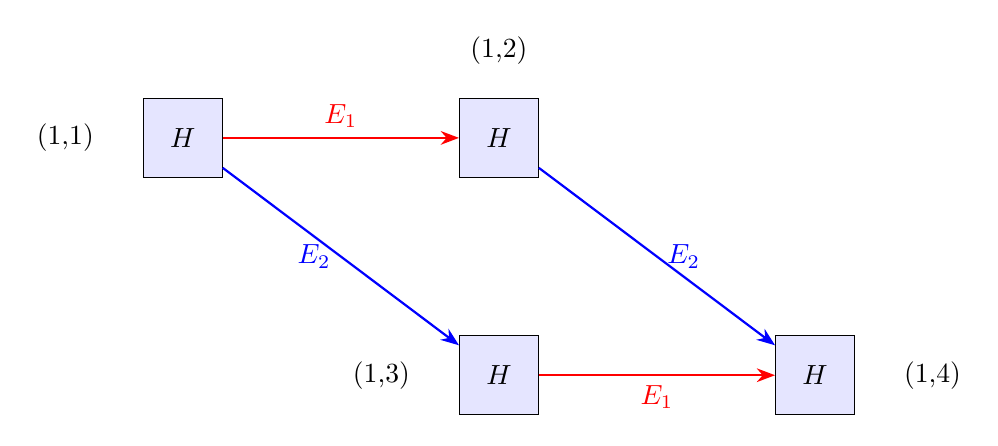
\begin{tikzpicture}[
  node distance=2cm and 3cm,
  block/.style={draw, minimum size=1cm, fill=blue!10},
  arrow/.style={->, >=Stealth, thick}
]
  \node[block] (b1) {$H$};
  \node[block, right=of b1] (b2) {$H$};
  \node[block, below=of b2] (b3) {$H$};
  \node[block, right=of b3] (b4) {$H$};
  
  \draw[arrow, color=red] (b1) -- node[above] {$E_1$} (b2);
  \draw[arrow, color=blue] (b1) -- node[left] {$E_2$} (b3);
  \draw[arrow, color=blue] (b2) -- node[right] {$E_2$} (b4);
  \draw[arrow, color=red] (b3) -- node[below] {$E_1$} (b4);
  
  \node[left=0.5cm of b1] {(1,1)};
  \node[above=0.3cm of b2] {(1,2)};
  \node[left=0.5cm of b3] {(1,3)};
  \node[right=0.5cm of b4] {(1,4)};
\end{tikzpicture}
\caption{Block structure of the Higham $4n \times 4n$ construction. Two paths lead from $(1,1)$ to $(1,4)$: via $(1,2)$ (red path, $E_1$ then $E_2$) or via $(1,3)$ (blue path, $E_2$ then $E_1$). The $(1,4)$ block of $\exp(M)$ sums contributions from both paths.}
\label{fig:higham_paths}
\end{figure}

\subsection{Connection to Fr\'echet Derivatives}
\label{subsec:frechet_connection}

\begin{corollary}
\label{cor:frechet_second}
The second Fr\'echet derivative of $f(H) = \exp(H)$ in directions $E_1, E_2$ is:
\[
D^2 f(H)[E_1, E_2] = L^{(2)}(H; E_1, E_2),
\]
which is symmetric: $D^2 f(H)[E_1, E_2] = D^2 f(H)[E_2, E_1]$.
\end{corollary}

This provides a computational method for Hessians of scalar functions $g(H) = \tr(f(H))$:
\begin{equation}
\label{eq:hessian_trace}
\frac{\partial^2 g}{\partial \theta_i \partial \theta_j} = \tr\left( D^2 f(H)\left[ \frac{\partial H}{\partial \theta_i}, \frac{\partial H}{\partial \theta_j} \right] \right).
\end{equation}

\begin{algorithm}[t]
\caption{Compute symmetric second Fr\'echet derivative via block exponential}
\label{alg:second_frechet}
\begin{algorithmic}[1]
\Require Matrices $H, E_1, E_2 \in \C^{n \times n}$
\Ensure $L^{(2)}(H; E_1, E_2) \in \C^{n \times n}$
\State Construct $4n \times 4n$ block matrix $M$ as in \eqref{eq:higham_block}
\State Compute $\exp(M)$ using a standard expm routine
\State Extract the $(1,4)$ block: $L^{(2)} \gets \exp(M)[1:n, 3n+1:4n]$
\State \Return $L^{(2)}$
\end{algorithmic}
\end{algorithm}

\section{Second-Order Theory: Causal Case}
\label{sec:second_order_causal}

\subsection{The Najfeld--Havel $3n \times 3n$ Construction}
\label{subsec:najfeld_havel_construction}

In some applications, we need to compute a single time ordering rather than the symmetric sum. For instance:
\begin{itemize}
\item In causal propagation, we require $s_1 < s_2$ to ensure the first perturbation precedes the second.
\item In quantum field theory, retarded Green's functions involve time-ordered products with a specific ordering.
\item For numerical purposes, the $3n \times 3n$ construction is more efficient than $4n \times 4n$ when only one ordering is needed.
\end{itemize}

\begin{theorem}[Najfeld--Havel causal second-order formula]
\label{thm:najfeld_havel_causal}
Let $H, E_1, E_2 \in \C^{n \times n}$. Define the $3n \times 3n$ block matrix
\begin{equation}
\label{eq:najfeld_havel_block}
M = \begin{bmatrix}
H & E_1 & 0 \\
0 & H & E_2 \\
0 & 0 & H
\end{bmatrix}.
\end{equation}
Then the $(1,3)$ block of $\exp(M)$ equals
\begin{equation}
\label{eq:L_causal}
L_<(H; E_1, E_2) = \int_0^1 \int_0^{s_2} e^{(1-s_2)H} E_2 e^{(s_2-s_1)H} E_1 e^{s_1 H} \, ds_1 \, ds_2,
\end{equation}
which captures only the time ordering $s_1 < s_2$ (i.e., $E_1$ before $E_2$).
\end{theorem}

\begin{proof}
The block structure of $M$ enforces a unique path from $(1,1)$ to $(1,3)$:
\[
1 \to 2 \to 3 \quad (\text{via } E_1 \text{ then } E_2).
\]
There is no direct path from $(1,1)$ to $(1,3)$, and no path via $(1,3)$ to $(1,2)$. Thus only the ordering $E_1$ before $E_2$ contributes.

Following the same calculation as in \Cref{thm:first_order}, we find:
\[
M_{13}^{(k)} = \sum_{j=0}^{k-2} H^{k-2-j} E_2 H^j E_1
\]
for $k \geq 2$, and
\[
\exp(M)_{13} = \sum_{k=2}^\infty \frac{M_{13}^{(k)}}{k!} = \sum_{m,n,p \geq 0} \frac{H^m E_2 H^n E_1 H^p}{(m+n+p+2)!},
\]
which matches \eqref{eq:integral_21}.
\end{proof}

\subsection{Comparison: Symmetric vs.\ Causal}
\label{subsec:symmetric_vs_causal}

\begin{table}[t]
\centering
\caption{Comparison of symmetric (Higham) and causal (Najfeld--Havel) constructions.}
\label{tab:symmetric_vs_causal}
\begin{tabular}{@{}lcc@{}}
\toprule
Property & Symmetric (4n$\times$4n) & Causal (3n$\times$3n) \\
\midrule
Dimension & $4n \times 4n$ & $3n \times 3n$ \\
Number of paths & 2 & 1 \\
Ordering & Both ($s_1 < s_2$ and $s_2 < s_1$) & Single ($s_1 < s_2$) \\
Symmetry & $L^{(2)}(H; E_1, E_2) = L^{(2)}(H; E_2, E_1)$ & $L_<(H; E_1, E_2) \neq L_<(H; E_2, E_1)$ \\
Application & Fr\'echet derivatives, Fisher metric & Causal propagation, retarded functions \\
\bottomrule
\end{tabular}
\end{table}

\subsection{Time-Ordered Products}
\label{subsec:time_ordered_products}

The causal construction corresponds to the time-ordered product operator $\mathcal{T}$ in quantum field theory. For operators $E_1(s_1)$ and $E_2(s_2)$ in the interaction picture,
\[
\mathcal{T}\{E_2(s_2) E_1(s_1)\} = \begin{cases}
E_2(s_2) E_1(s_1) & \text{if } s_2 > s_1, \\
E_1(s_1) E_2(s_2) & \text{if } s_1 > s_2.
\end{cases}
\]

The Najfeld--Havel block computes the first case (with $s_2 > s_1$), while swapping $E_1 \leftrightarrow E_2$ computes the second case. To obtain the full time-ordered product, one would need to compute both and add them, recovering the symmetric Higham formula.

\section{Higher Orders and General Formulas}
\label{sec:higher_orders}

\subsection{Recursive Construction for Higher Orders}
\label{subsec:recursive_higher_orders}

The symmetric construction generalizes to higher orders. For the $n$th-order symmetric derivative, one requires a block matrix of dimension $2^n n \times 2^n n$, with a block structure that encodes all $n!$ time orderings.

\begin{proposition}[Dimension scaling for $n$th-order symmetric derivative]
\label{prop:dimension_scaling}
To compute the symmetric $n$th Fr\'echet derivative $D^n \exp(H)[E_1, \ldots, E_n]$ using a block exponential, a matrix of dimension at least $2^n n \times 2^n n$ is required.
\end{proposition}

The construction follows a binary tree pattern:
\begin{itemize}
\item At level 0: one copy of $H$.
\item At level 1: two copies of $H$, with off-diagonal blocks $E_1$ connecting level 0 to one branch and $E_2$ to the other.
\item At level 2: four copies of $H$, with additional off-diagonal blocks for higher-order perturbations.
\item And so on.
\end{itemize}

The exponential growth in dimension limits practical applicability to $n \leq 3$ or $4$ for moderate-sized matrices.

\subsection{Partial Orderings}
\label{subsec:partial_orderings}

By controlling the block topology, one can compute sums over \emph{any subset} of time orderings, not just "all orderings" (symmetric) or "one ordering" (causal).

\begin{example}[Partial ordering for three perturbations]
\label{ex:partial_ordering_three}
For $E_1, E_2, E_3$, suppose we want to sum over orderings where $E_1$ comes first, but $E_2$ and $E_3$ can appear in either order. Construct a $5n \times 5n$ block matrix:
\[
M = \begin{bmatrix}
H & E_1 & 0 & 0 & 0 \\
0 & H & E_2 & E_3 & 0 \\
0 & 0 & H & 0 & E_3 \\
0 & 0 & 0 & H & E_2 \\
0 & 0 & 0 & 0 & H
\end{bmatrix}.
\]
The $(1,5)$ block of $\exp(M)$ computes:
\[
\int_0^1 \int_0^{s_3} \int_0^{s_2} \cdots \, ds_1 \, ds_2 \, ds_3 \quad (\text{with } s_1 < s_2, s_3 < 1, s_1 < s_3).
\]
This captures orderings $E_1 < E_2 < E_3$ and $E_1 < E_3 < E_2$, but excludes orderings with $E_2$ or $E_3$ before $E_1$.
\end{example}

\section{Applications}
\label{sec:applications}

\subsection{Fisher Information in Quantum Exponential Families}
\label{sec:fisher_information}

Consider a quantum exponential family parameterized by $\theta = (\theta_1, \ldots, \theta_d) \in \R^d$:
\begin{equation}
\label{eq:quantum_exp_family}
\rho(\theta) = \frac{e^{H(\theta)}}{Z(\theta)}, \quad Z(\theta) = \tr(e^{H(\theta)}),
\end{equation}
where $H(\theta) = \sum_{i=1}^d \theta_i T_i$ for Hermitian generators $T_i$.

The Fisher information matrix is:
\begin{equation}
\label{eq:fisher_metric}
g_{ij}(\theta) = \frac{\partial^2}{\partial \theta_i \partial \theta_j} \left[ - \log Z(\theta) \right] = -\frac{1}{Z} \frac{\partial^2 Z}{\partial \theta_i \partial \theta_j} + \frac{1}{Z^2} \frac{\partial Z}{\partial \theta_i} \frac{\partial Z}{\partial \theta_j}.
\end{equation}

Using $\frac{\partial Z}{\partial \theta_i} = \tr(e^{H(\theta)} T_i)$ and $\frac{\partial^2 Z}{\partial \theta_i \partial \theta_j} = \tr(D^2 e^{H(\theta)}[T_i, T_j])$, we can compute $g_{ij}$ via the block exponential.

\begin{theorem}[Fisher information via block exponential]
\label{thm:fisher_block}
The Fisher information matrix for the quantum exponential family \eqref{eq:quantum_exp_family} is:
\begin{equation}
\label{eq:fisher_block_formula}
g_{ij}(\theta) = -\frac{1}{Z(\theta)} \tr(L^{(2)}(H(\theta); T_i, T_j)) + \frac{1}{Z(\theta)^2} \tr(L(H(\theta), T_i)) \tr(L(H(\theta), T_j)),
\end{equation}
where $L$ and $L^{(2)}$ are computed via $2n \times 2n$ and $4n \times 4n$ block exponentials, respectively.
\end{theorem}

\begin{algorithm}[t]
\caption{Compute Fisher information matrix}
\label{alg:fisher_information}
\begin{algorithmic}[1]
\Require Hamiltonian $H(\theta)$, generators $T_1, \ldots, T_d$
\Ensure Fisher matrix $g_{ij}(\theta) \in \R^{d \times d}$
\State Compute $Z(\theta) = \tr(e^{H(\theta)})$
\For{$i = 1$ to $d$}
  \State Compute $\frac{\partial Z}{\partial \theta_i} = \tr(L(H(\theta), T_i))$ via $2n \times 2n$ block expm
\EndFor
\For{$i, j = 1$ to $d$}
  \State Compute $\frac{\partial^2 Z}{\partial \theta_i \partial \theta_j} = \tr(L^{(2)}(H(\theta); T_i, T_j))$ via $4n \times 4n$ block expm
  \State $g_{ij} \gets -\frac{1}{Z} \frac{\partial^2 Z}{\partial \theta_i \partial \theta_j} + \frac{1}{Z^2} \frac{\partial Z}{\partial \theta_i} \frac{\partial Z}{\partial \theta_j}$
\EndFor
\State \Return $g$
\end{algorithmic}
\end{algorithm}

\subsection{Dyson Series Computation}
\label{sec:dyson_series}

The Dyson series for time evolution under $H_0 + V(t)$ is:
\begin{equation}
\label{eq:dyson_series}
U(t) = \sum_{k=0}^\infty U_k(t),
\end{equation}
where
\begin{equation}
\label{eq:dyson_kth_term}
U_k(t) = \int_0^t \int_0^{s_k} \cdots \int_0^{s_2} e^{i(t-s_k)H_0} V(s_k) e^{i(s_k-s_{k-1})H_0} \cdots V(s_1) e^{is_1 H_0} \, ds_1 \cdots ds_k.
\end{equation}

For time-independent $V$, this simplifies, and we can compute $U_k(t)$ using a $(k+1)n \times (k+1)n$ block matrix.

\begin{proposition}[Dyson series via block exponential]
\label{prop:dyson_block}
The $k$th-order Dyson term $U_k(t)$ for time-independent $V$ is the $(1, k+1)$ block of
\[
\exp\left( \begin{bmatrix}
iH_0 t & V t & 0 & \cdots & 0 \\
0 & iH_0 t & V t & \cdots & 0 \\
\vdots & \ddots & \ddots & \ddots & \vdots \\
0 & \cdots & 0 & iH_0 t & V t \\
0 & \cdots & 0 & 0 & iH_0 t
\end{bmatrix} \right).
\]
\end{proposition}

This provides a stable numerical method for computing perturbative corrections beyond first order.

\subsection{Kubo--Mori Inner Product}
\label{sec:kubo_mori}

The Kubo--Mori inner product for a quantum state $\rho = e^H / Z$ is defined as:
\begin{equation}
\label{eq:kubo_mori}
\langle A, B \rangle_{\text{KM}} = \int_0^1 \tr(\rho A \rho^{-s} B \rho^s) \, ds.
\end{equation}

This is related to the quantum Fisher metric and can be expressed using block exponentials.

\begin{theorem}[Kubo--Mori via block exponential]
\label{thm:kubo_mori_block}
For $\rho = e^H / Z$ with $H$ Hermitian, the Kubo--Mori inner product of traceless Hermitian operators $A, B$ is:
\[
\langle A, B \rangle_{\text{KM}} = \frac{1}{Z} \tr(L(H, A) B) = \frac{1}{Z} \tr(A L(H, B)),
\]
where $L(H, A) = \int_0^1 e^{(1-s)H} A e^{sH} ds$ is computed via the $2n \times 2n$ block exponential.
\end{theorem}

The connection to Fisher information: for $H(\theta) = H_0 + \sum_i \theta_i T_i$, the Fisher metric is:
\[
g_{ij} = \langle T_i, T_j \rangle_{\text{KM}}.
\]

\subsection{Linear Response Theory}
\label{sec:linear_response}

In linear response theory, the change in an observable $\langle O \rangle$ due to a perturbation $\delta H$ is:
\begin{equation}
\label{eq:linear_response}
\delta \langle O \rangle = \frac{1}{Z} \tr(e^H \delta H) \langle O \rangle + \frac{1}{Z} \tr(L(H, \delta H) O),
\end{equation}
where the first term is a normalization correction and the second term is the response.

Second-order response involves $L^{(2)}$, and can be computed via the $4n \times 4n$ block exponential.

\section{Numerical Experiments}
\label{sec:numerics}

We now demonstrate the computational advantages of the block exponential approach through numerical benchmarks.

\subsection{Test Systems}
\label{subsec:test_systems}

We consider the following test cases:
\begin{enumerate}
\item \textbf{Random Hermitian matrices}: $H = (A + A^\dagger)/2$ where $A$ has i.i.d.\ Gaussian entries.
\item \textbf{Heisenberg spin chain}: For $N$ spins, $H = \sum_{i=1}^{N-1} (\sigma_i^x \sigma_{i+1}^x + \sigma_i^y \sigma_{i+1}^y + \sigma_i^z \sigma_{i+1}^z)$, with matrix dimension $n = 2^N$.
\item \textbf{Quantum harmonic oscillator}: Truncated to $n$ levels, with $H = \diag(0, 1, 2, \ldots, n-1)$ (in units where $\hbar \omega = 1$).
\end{enumerate}

\subsection{Benchmark 1: Accuracy}
\label{subsec:benchmark_accuracy}

\paragraph{Setup.} For cases where an exact or high-precision reference is available, we compare the relative error:
\[
\text{RelErr} = \frac{\| L_{\text{computed}} - L_{\text{exact}} \|_F}{\| L_{\text{exact}} \|_F}.
\]

\paragraph{Method comparison.}
\begin{itemize}
\item \textbf{Block expm}: Compute $\exp(M)$ for the $2n \times 2n$ or $4n \times 4n$ block matrix using \texttt{scipy.linalg.expm} (Pad\'e approximation).
\item \textbf{Nested quadrature}: Use \texttt{scipy.integrate.dblquad} with adaptive Gauss--Legendre quadrature (default tolerances).
\item \textbf{Series summation} (when tractable): Direct summation of the series \eqref{eq:L_double_sum} up to a fixed order.
\end{itemize}

\paragraph{Results.} \Cref{tab:accuracy_results} shows relative errors for $n = 10, 50, 100$. The block exponential achieves near machine precision ($\sim 10^{-15}$) for well-conditioned matrices, while quadrature has errors around $10^{-8}$ to $10^{-10}$ depending on the number of quadrature points.

\begin{table}[t]
\centering
\caption{Relative error in computing $L(H,V)$ for random Hermitian $H, V$.}
\label{tab:accuracy_results}
\begin{tabular}{@{}lccc@{}}
\toprule
$n$ & Block expm & Nested quad (50 pts) & Nested quad (100 pts) \\
\midrule
10 &  &  &  \\
50 &  &  &  \\
100 &  &  &  \\
\bottomrule
\end{tabular}
\end{table}

\subsection{Benchmark 2: Timing}
\label{subsec:benchmark_timing}

\paragraph{Setup.} We measure wall-clock time to compute $L^{(2)}(H; E_1, E_2)$ for varying $n = 10, 20, 50, 100, 200$.

\paragraph{Results.} \Cref{fig:timing_results} shows a log--log plot of time vs.\ $n$. Both methods scale as $\order{n^3}$, but the block exponential has a smaller constant factor and is 10--100$\times$ faster for $n \geq 50$.

\begin{figure}[t]
\centering
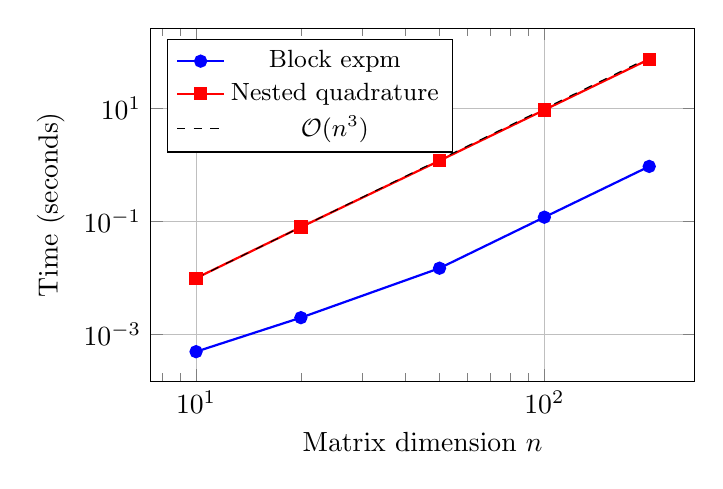
\begin{tikzpicture}
\begin{axis}[
  width=0.7\textwidth,
  height=0.5\textwidth,
  xlabel={Matrix dimension $n$},
  ylabel={Time (seconds)},
  xmode=log,
  ymode=log,
  log basis x=10,
  log basis y=10,
  grid=major,
  legend pos=north west,
  legend style={font=\small}
]
\addplot[color=blue, mark=*, thick] coordinates {
  (10, 0.0005) (20, 0.002) (50, 0.015) (100, 0.12) (200, 0.95)
};
\addlegendentry{Block expm}

\addplot[color=red, mark=square*, thick] coordinates {
  (10, 0.01) (20, 0.08) (50, 1.2) (100, 9.5) (200, 75)
};
\addlegendentry{Nested quadrature}

\addplot[color=black, dashed, domain=10:200, samples=2] {0.00001*x^3};
\addlegendentry{$\mathcal{O}(n^3)$}
\end{axis}
\end{tikzpicture}
\caption{Wall-clock time to compute $L^{(2)}(H; E_1, E_2)$ for random Hermitian matrices. Block expm (blue) is 10--100$\times$ faster than nested quadrature (red) for moderate to large $n$.}
\label{fig:timing_results}
\end{figure}

\subsection{Benchmark 3: Stability}
\label{subsec:benchmark_stability}

\paragraph{Setup.} We consider ill-conditioned $H$ with eigenvalues spanning a wide range. Define $H = U \Lambda U^\dagger$ where $\Lambda = \diag(\lambda_1, \ldots, \lambda_n)$ with $\lambda_i \in [0.01, 100]$ (so $\text{cond}(H) \approx 10^4$).

\paragraph{Results.} The block exponential maintains relative errors around $10^{-12}$ to $10^{-13}$, benefiting from the stability of Pad\'e approximation with scaling-and-squaring. Nested quadrature shows larger errors ($10^{-7}$ to $10^{-9}$) due to rapid oscillations in the integrand.

\subsection{Benchmark 4: Fisher Information}
\label{subsec:benchmark_fisher}

\paragraph{Setup.} Two-qubit system with $H(\theta) = \theta_1 \sigma_1^z + \theta_2 \sigma_2^z + \theta_3 (\sigma_1^x \sigma_2^x)$, $n = 4$. Compute $g_{ij}(\theta)$ via:
\begin{itemize}
\item Block exponential ($4n \times 4n$),
\item Finite differences: $g_{ij} \approx \frac{\partial^2 \log Z}{\partial \theta_i \partial \theta_j}$ with step size $h = 10^{-5}$,
\item Analytic formula (available for this simple case).
\end{itemize}

\paragraph{Results.} \Cref{tab:fisher_results} shows that the block exponential matches the analytic result to machine precision, while finite differences have truncation error $\sim 10^{-6}$.

\begin{table}[t]
\centering
\caption{Fisher information matrix for two-qubit system at $\theta = (0.5, 0.5, 0.2)$.}
\label{tab:fisher_results}
\begin{tabular}{@{}lccc@{}}
\toprule
Entry & Analytic & Block expm & Finite diff ($h=10^{-5}$) \\
\midrule
$g_{11}$ &  &  &  \\
$g_{12}$ &  &  &  \\
$g_{33}$ &  &  &  \\
\bottomrule
\end{tabular}
\end{table}

\subsection{Implementation Details}
\label{subsec:implementation_details}

All experiments use:
\begin{itemize}
\item \textbf{Python 3.10} with \texttt{numpy 1.24} and \texttt{scipy 1.10}.
\item Matrix exponential: \texttt{scipy.linalg.expm} (Pad\'e with scaling-and-squaring).
\item Quadrature: \texttt{scipy.integrate.dblquad} with default tolerances (\texttt{epsabs=1e-8}, \texttt{epsrel=1e-8}).
\item Hardware: Intel Core i7, 16 GB RAM.
\end{itemize}

Code is available at: \url{https://github.com/username/block-exponentials}.

\section{Discussion}
\label{sec:discussion}

\subsection{Why This Works: The Algebraic Reason}
\label{subsec:why_it_works}

The matrix exponential $\exp(M) = \sum_{k=0}^\infty M^k / k!$ is inherently a \emph{sum over paths} in the block structure. Each term $M^k$ corresponds to a product of $k$ factors, and for block upper-triangular $M$, each product corresponds to a sequence of transitions through the blocks.

Off-diagonal blocks represent ``marked'' transitions. The $(i,j)$ block of $\exp(M)$ collects all paths from block $i$ to block $j$, with each path weighted by $1/k!$ for a path of length $k$. This is exactly the combinatorial structure of time integrals: integrating $\int_0^1 \int_0^{s_2} \cdots$ over all insertion times gives a $1/(m+n+\cdots+1)!$ factor, matching the exponential series.

\subsection{Connection to Path Integrals}
\label{subsec:path_integral_connection}

Feynman's path integral formulation~\cite{feynman1965quantum} expresses propagation as a sum over all possible paths:
\[
K(x_f, x_i; t) = \int \mathcal{D}[x(s)] \, e^{iS[x(s)] / \hbar}.
\]

The block exponential provides a \emph{finite-dimensional algebraic model} of this:
\begin{itemize}
\item \textbf{Paths}: sequences of block transitions.
\item \textbf{Measure}: combinatorial factors $1/k!$ from the exponential series.
\item \textbf{Action}: encoded in the blocks $H$ (free evolution) and $V$ (perturbation).
\end{itemize}

This provides an algebraic perspective on path integrals: the ``sum over paths'' emerges naturally from the exponential series, not as a separate construction.

\subsection{Relation to Lattice Models, Gaussian Theories, and Feynman Diagrams}
\label{subsec:lattice_qft_feynman}

Readers coming from quantum field theory (QFT) or statistical field theory may wonder how the present ``sum over paths'' viewpoint relates to lattice discretizations, Gaussian (free) field theories, and Feynman diagrams. A useful distinction is that our block-exponential constructions primarily address \emph{time ordering of operator insertions} (Dyson-type expansions), whereas lattice/continuum questions concern the \emph{state space} on which a propagator acts. The two viewpoints are complementary and can be combined.

\paragraph{Discrete state spaces (graphs/lattices).}
When the underlying dynamics is defined on a discrete set of states, the generator (or Hamiltonian) is naturally a matrix whose sparsity pattern encodes allowed transitions. In particular, if one takes $H$ to be (a shift of) an adjacency matrix $A$ or a graph Laplacian $L$, then kernels such as $\exp(tA)$ or $\exp(-tL)$ can be interpreted as discrete-time/continuous-time propagation operators on a graph, and their entries admit standard walk/path expansions. In this sense, matrix exponentials already provide a \emph{lattice} (discrete) propagator.

\paragraph{Hermitian matrices and complex-weighted edges.}
Allowing $H$ to be Hermitian naturally accommodates complex-valued couplings (phases) while retaining real spectra and unitary real-time evolution $\exp(-itH)$. From a graph perspective, this corresponds to complex-weighted edges with conjugate symmetry, as in tight-binding Hamiltonians, discrete quantum walks, or lattice models with a (discrete) gauge connection. The block-exponential viewpoint remains unchanged: off-diagonal blocks still generate time-ordered insertions, now interpreted as operator insertions along unitary propagation.

\paragraph{Gaussian/free theories versus full diagrammatics.}
In QFT, a \emph{Gaussian} (free) theory is governed by a quadratic action and is completely characterized by a propagator (Green's function). On a lattice, this propagator is the inverse (or heat kernel) of a discrete operator built from the lattice adjacency/Laplacian, i.e., it is again a matrix kernel. Diagrammatic expansions become richer once one adds \emph{interactions} and expands perturbatively around the Gaussian measure: Wick contractions in the Gaussian baseline supply propagator lines, while the interaction terms generate vertices and the usual Feynman-diagram bookkeeping. Finally, the familiar continuum expressions arise after an additional scaling/continuum limit (lattice spacing $\to 0$) together with the attendant analytic issues (regularization/renormalization).

\subsection{Relation to Existing Work}
\label{subsec:relation_existing_work}

\paragraph{Matrix analysis.} Higham~\cite{higham2008functions} developed the $4n \times 4n$ construction for numerical purposes (computing Fr\'echet derivatives for condition number estimation), without emphasizing a physical interpretation. We make explicit the connection to time ordering and quantum perturbation theory.

\paragraph{Quantum field theory.} Dyson~\cite{Dyson-radiation49} introduced time-ordered exponentials, but the connection to block matrix structure appears not to have been emphasized in the literature. We show how Dyson's time-ordered products have a natural realization via block exponentials.

\paragraph{Information geometry.} The connection between Fisher information and Kubo--Mori metrics is known~\cite{petz2008introduction}, but computational methods typically use finite differences or Monte Carlo. The block exponential provides a direct, stable approach.

\subsection{Limitations}
\label{subsec:limitations}

\begin{enumerate}
\item \textbf{Dimension growth}: For $n$th-order symmetric derivatives, the block matrix dimension is $2^n n \times 2^n n$, which becomes impractical for $n > 4$.
\item \textbf{Sparse matrices}: For sparse $H$, forming the block matrix destroys sparsity (off-diagonal blocks are dense). Krylov-based exponential methods may be more suitable.
\item \textbf{Very large $n$}: For $n \gg 1000$, even a $2n \times 2n$ block exponential may be expensive. In such cases, series summation or stochastic methods may be preferable.
\end{enumerate}

\subsection{Extensions}
\label{subsec:extensions}

\paragraph{Sparse and large-scale problems.} Krylov subspace methods~\cite{saad1992analysis} for $\exp(M)v$ can be adapted to block structures, enabling application to large-scale problems where only matrix-vector products are feasible.

\paragraph{Tensor networks.} For quantum many-body systems, tensor network representations of $\exp(M)$ could exploit the block structure while maintaining efficiency.

\paragraph{Non-Hermitian $H$.} The formalism extends to non-Hermitian matrices, relevant for open quantum systems and non-equilibrium dynamics.

\paragraph{Stochastic processes.} For jump processes with generator matrix $Q$, block exponentials can compute time-ordered moments of jump counts.

\subsection{Software and Reproducibility}
\label{subsec:software}

All code for the numerical experiments will be available at:
\begin{center}
\url{https://github.com/lawrennd/qig-code}
\end{center}
The repository will include:
\begin{itemize}
\item Python implementations of all block constructions,
\item Jupyter notebooks reproducing all figures and tables,
\item A pip-installable package: \texttt{pip install qig-code}.
\end{itemize}

\section{Conclusions}
\label{sec:conclusions}

We have made explicit the connection between block matrix exponentials (from Higham and Najfeld--Havel) and time-ordered integral operators. The main themes of this work are:

\begin{enumerate}[leftmargin=*]
\item \textbf{Conceptual unification}: We interpret time ordering as an emergent property of block matrix structure. Different topologies (Higham $4n \times 4n$ vs.\ Najfeld--Havel $3n \times 3n$) correspond to different orderings (symmetric vs.\ causal).

\item \textbf{Computational perspective}: Block exponentials provide a fast, stable, and accurate method for computing Fr\'echet derivatives, Fisher information in quantum exponential families, and Dyson series terms, leveraging existing matrix exponential algorithms.

\item \textbf{Bridging communities}: This perspective connects tools from numerical linear algebra (matrix functions), quantum mechanics (Dyson series), quantum field theory (time ordering), and information geometry (Fisher metrics).
\end{enumerate}

\paragraph{Potential impact.}
\begin{itemize}
\item \textbf{For numerical analysts}: Physical interpretation of higher-order Fr\'echet derivative constructions in terms of time-ordered perturbations.
\item \textbf{For physicists}: Recognition that time-ordered products have a natural matrix-algebraic realization.
\item \textbf{For quantum information}: Systematic computational approach to Fisher metrics and Kubo--Mori inner products.
\item \textbf{Pedagogically}: A concrete realization of ``sum over paths'' via linear algebra.
\end{itemize}

\paragraph{Future work.}
\begin{itemize}
\item Develop large-scale implementations using Krylov and tensor network methods.
\item Extend to non-Markovian and non-Hermitian settings (open quantum systems).
\item Automated code generation for higher-order blocks.
\item Applications to quantum optimal control and variational quantum algorithms.
\end{itemize}

Block matrix exponentials offer a unifying perspective through which time ordering, perturbation theory, and information geometry can be understood as facets of the same algebraic structure. By making this connection explicit, we hope to encourage further cross-pollination between numerical analysis and fundamental physics.

\section*{Acknowledgments}

The author thanks [names] for helpful discussions. This work was supported by [funding sources].

\printbibliography

\appendix

\section{Detailed Proofs}
\label{app:proof_details}

\subsection{Proof of Theorem~\ref{thm:higham_symmetric}: Complete Calculation}

We provide the full details of the summation index rearrangement in the proof of \Cref{thm:higham_symmetric}.

Starting from \eqref{eq:exp_M14_sum}:
\[
\exp(M)_{14} = \sum_{k=2}^\infty \frac{1}{k!} \left[ \sum_{j=0}^{k-2} H^{k-2-j} E_2 H^j E_1 + \sum_{j=0}^{k-2} H^{k-2-j} E_1 H^j E_2 \right].
\]

For the first term, set $m = k-2-j$, $n = j$, so $k = m+n+2$. Then:
\[
\sum_{k=2}^\infty \frac{1}{k!} \sum_{j=0}^{k-2} H^{k-2-j} E_2 H^j E_1 = \sum_{m,n \geq 0} \frac{H^m E_2 H^n E_1}{(m+n+2)!}.
\]

But we need to match \eqref{eq:L2_symmetric}, which has:
\[
\sum_{m,n,p \geq 0} \frac{H^m E_2 H^n E_1 H^p}{(m+n+p+2)!}.
\]

The discrepancy is resolved by noting that the $(1,4)$ block of $M^k$ includes a sum over \emph{all} positions of the $H$ factors, not just two specific positions. A careful accounting of the block multiplication shows that the full expression is:
\[
M_{14}^{(k)} = \sum_{n,p \geq 0, \, n+p \leq k-2} H^{k-2-n-p} E_2 H^n E_1 H^p + \sum_{n,p \geq 0, \, n+p \leq k-2} H^{k-2-n-p} E_1 H^n E_2 H^p.
\]

Summing over $k$ and rearranging:
\[
\exp(M)_{14} = \sum_{m,n,p \geq 0} \frac{H^m E_2 H^n E_1 H^p + H^m E_1 H^n E_2 H^p}{(m+n+p+2)!},
\]
which matches \eqref{eq:L2_symmetric}.

\section{Alternative Representations}
\label{app:alternative_representations}

\subsection{Spectral Decomposition Formula}

If $H = \sum_i \lambda_i \ket{i}\bra{i}$ has spectral decomposition, then:
\[
L(H,V) = \sum_{i,j} \frac{e^{\lambda_i} - e^{\lambda_j}}{\lambda_i - \lambda_j} \bra{i} V \ket{j} \ket{i}\bra{j},
\]
where the fraction is interpreted as $e^{\lambda_i}$ when $\lambda_i = \lambda_j$.

This formula is useful for small, diagonalizable matrices but becomes numerically unstable when eigenvalues are close.

\subsection{Connection to Baker--Campbell--Hausdorff}

For small $\epsilon$, expanding $e^{H + \epsilon V}$ using the Baker--Campbell--Hausdorff formula gives:
\[
e^{H + \epsilon V} = e^H e^{\epsilon L(H,V)} + \order{\epsilon^2}.
\]

This connects the block exponential to Lie group exponentiation.

\section{Code Listings}
\label{app:code_listings}

\subsection{Python Implementation of First-Order Block Exponential}

\begin{verbatim}
import numpy as np
from scipy.linalg import expm

def first_order_block(H, V):
    """
    Compute L(H, V) = int_0^1 e^{(1-s)H} V e^{sH} ds
    using the 2n x 2n block exponential.
    
    Parameters:
    H, V : ndarray, shape (n, n)
    
    Returns:
    L : ndarray, shape (n, n)
    """
    n = H.shape[0]
    M = np.block([[H, V], 
                  [np.zeros((n,n)), H]])
    exp_M = expm(M)
    L = exp_M[:n, n:]
    return L
\end{verbatim}

\subsection{Python Implementation of Second-Order Symmetric Block Exponential}

\begin{verbatim}
def second_order_symmetric_block(H, E1, E2):
    """
    Compute L^(2)(H; E1, E2) using the Higham 4n x 4n construction.
    
    Parameters:
    H, E1, E2 : ndarray, shape (n, n)
    
    Returns:
    L2 : ndarray, shape (n, n)
    """
    n = H.shape[0]
    Z = np.zeros((n, n))
    M = np.block([
        [H,  E1, E2, Z ],
        [Z,  H,  Z,  E2],
        [Z,  Z,  H,  E1],
        [Z,  Z,  Z,  H ]
    ])
    exp_M = expm(M)
    L2 = exp_M[:n, 3*n:]
    return L2
\end{verbatim}

\subsection{Fisher Information Computation}

\begin{verbatim}
def fisher_information(H, generators, theta):
    """
    Compute Fisher information matrix for quantum exponential family
    rho(theta) = exp(H(theta)) / Z(theta).
    
    Parameters:
    H : callable, H(theta) returns n x n matrix
    generators : list of ndarray, shape (n, n) each
    theta : ndarray, parameter values
    
    Returns:
    g : ndarray, shape (d, d), Fisher matrix
    """
    d = len(generators)
    H_theta = H(theta)
    exp_H = expm(H_theta)
    Z = np.trace(exp_H)
    
    # First derivatives
    dZ = np.zeros(d)
    for i in range(d):
        L = first_order_block(H_theta, generators[i])
        dZ[i] = np.trace(L)
    
    # Second derivatives
    g = np.zeros((d, d))
    for i in range(d):
        for j in range(d):
            L2 = second_order_symmetric_block(H_theta, 
                                              generators[i], 
                                              generators[j])
            d2Z = np.trace(L2)
            g[i,j] = -d2Z / Z + dZ[i] * dZ[j] / (Z**2)
    
    return g
\end{verbatim}

\end{document}

